% Informe técnico de la Pregunta 1 del examen parcial (Redes Neuronales 2026-II, FIIS-UNI).
% Formato: plantilla IEEE del curso (docs/Plantilla_Paper_IEEE-1.pdf), IEEEtran en modo conferencia.
% Fuentes de los números: output-data/ (corrida 1, semilla 42) y output-data-v2/semillas.csv (corrida 2, semillas 42, 1 y 2).
% Compilar: tectonic main.tex   (o pdflatex + bibtex en Overleaf)
\documentclass[conference]{IEEEtran}

\usepackage{iftex}
\ifTUTeX % XeTeX/LuaTeX (tectonic): Times como en la plantilla
  \usepackage{fontspec}
  \setmainfont{texgyretermes}[Extension=.otf, UprightFont=*-regular, BoldFont=*-bold,
    ItalicFont=*-italic, BoldItalicFont=*-bolditalic]
\else % pdfLaTeX (Overleaf)
  \usepackage[utf8]{inputenc}
  \usepackage[T1]{fontenc}
\fi
\usepackage[spanish,es-tabla,es-nodecimaldot]{babel}
\usepackage{cite}
\usepackage{amsmath,amssymb}
\usepackage{booktabs}
\usepackage{graphicx}
\usepackage{tikz}
\usetikzlibrary{positioning,babel} % babel: los atajos de español rompen las flechas de TikZ
\usepackage[hidelinks]{hyperref}

\renewcommand{\IEEEkeywordsname}{Palabras clave}

\begin{document}

\title{Detección multietiqueta de anomalías de rodilla en resonancia magnética con una CNN 2.5D y atención, entrenada con etiquetas débiles de reportes multilingües}

% Cuatro integrantes en dos filas de dos. Correos pendientes: agregarlos como última línea de cada \IEEEauthorblockA.
\makeatletter
\newcommand{\linebreakand}{\end{@IEEEauthorhalign}\hfill\mbox{}\par\mbox{}\hfill\begin{@IEEEauthorhalign}}
\makeatother
\newcommand{\afiliacion}{\IEEEauthorblockA{\textit{Maestría en Inteligencia Artificial}\\ FIIS -- UNI\\ Lima, Perú}}
\author{%
  \IEEEauthorblockN{Burgos Choquehuanca Juan}\afiliacion
  \and
  \IEEEauthorblockN{Paredes Abanto Davis Roberto}\afiliacion
  \linebreakand
  \IEEEauthorblockN{Salguero Torres Carlos Adrian}\afiliacion
  \and
  \IEEEauthorblockN{Ramirez Quispe Huber Angel}\afiliacion
}

\maketitle

\begin{abstract}
Leer una resonancia magnética de rodilla exige un especialista, y entrenar un modelo que lo asista exige etiquetas expertas que casi nunca existen: en la competencia RSNA Knee Abnormality Detection solo 58 de 4407 estudios las tienen.
Este trabajo convierte los reportes radiológicos, escritos en al menos nueve idiomas, en etiquetas débiles para 12 hallazgos mediante un extractor de reglas con detección de negación y duda, y con ellas entrena una red 2.5D: una CNN procesa ventanas de tres cortes vecinos de cada plano, dos bloques de autoatención combinan las ventanas y una consulta de atención por hallazgo produce 12 probabilidades independientes.
Los 58 estudios con etiqueta experta se reservan para la evaluación.
Con tres semillas, ResNet-18 preentrenada en ImageNet alcanza un AUC macro de 0.732 ± 0.010 frente a 0.595 ± 0.006 de una CNN entrenada desde cero, la única diferencia significativa; la pérdida focal mejora a la referencia en las tres semillas (0.742 ± 0.007), aunque sin significancia estadística.
El modelo de imagen queda cerca del extractor que generó sus etiquetas (0.753) y lo supera en derrame, artrosis medial y contusión.
Se concluye que el cuello de botella es la supervisión y no la arquitectura: las etiquetas subestiman los hallazgos que el radiólogo no escribe, y Grad-CAM muestra que el modelo aprovecha co-ocurrencias del reporte.
\end{abstract}

\begin{IEEEkeywords}
aprendizaje profundo, resonancia magnética de rodilla, supervisión débil, clasificación multietiqueta, atención, Grad-CAM
\end{IEEEkeywords}

% ---------------------------------------------------------------------------
\section{Introducción}
\label{sec:intro}

La resonancia magnética (RM) es el estudio de referencia para las lesiones de ligamentos, meniscos, cartílago y hueso de la rodilla.
Cada estudio tiene entre 3 y 14 series, en tres planos y con distintas secuencias, y su lectura requiere un radiólogo con experiencia musculoesquelética.
Un sistema que priorice los estudios con hallazgos podría reducir los tiempos de espera donde ese especialista escasea.
El obstáculo es la supervisión: los hospitales guardan millones de estudios con su reporte en texto libre, pero casi ninguno con etiquetas estructuradas.
Además, los reportes están en el idioma de cada centro; en un país como el Perú, un sistema así tendría que aprender de reportes en español, que, como se verá, son los que más información dejan implícita.

\paragraph*{Formulación}
La competencia RSNA Knee Abnormality Detection~\cite{rsna2026knee} define la entrada como un estudio de RM de rodilla (todas sus series DICOM) y la salida como 12 probabilidades: rotura del ligamento cruzado anterior (ACL) y del colateral medial (MCL), rotura de menisco medial y lateral, artrosis medial, lateral y patelofemoral (PF OA), derrame, sinovitis, quiste de Baker, contusión y fractura.
El éxito se mide con el AUC-ROC macro, el promedio de los 12 AUC.
De los 4407 estudios de entrenamiento, solo 58 tienen las 12 etiquetas de un experto (\emph{gold}); el resto trae únicamente el reporte.
Los estudios de prueba no traen reporte, así que el modelo final debe predecir solo a partir de la imagen.

\paragraph*{Por qué aprendizaje profundo y por qué esta arquitectura}
Los hallazgos son patrones visuales locales (una rotura, un edema, un quiste) que aparecen en pocos cortes de un plano concreto; no hay rasgos manuales que los capturen.
Una CNN es el extractor natural para cada corte, y el preentrenamiento en ImageNet compensa que solo se entrene con cientos de estudios.
Como el número de cortes y de planos varía y cada hallazgo se ve mejor en planos distintos, los rasgos de los cortes se combinan con autoatención~\cite{vaswani2017attention} y se agregan con una consulta de atención por hallazgo, de modo que cada salida elige sus propios cortes.

\paragraph*{Qué es nuevo respecto de los ejemplos del curso}
Los laboratorios del curso usan imágenes 2D con etiquetas limpias (VGG, GoogLeNet, U-Net, YOLO) y el Transformer sobre secuencias de texto.
Aquí la entrada es un volumen multiplano sin etiquetas, de modo que hay que construir la supervisión desde texto multilingüe, y se combinan una CNN por corte con autoatención escrita a mano entre cortes y planos.

Las contribuciones de este trabajo son:
\begin{itemize}
  \item Un extractor de etiquetas débiles multilingüe, validado contra los 58 gold, con un análisis de su ruido por hallazgo y de su sesgo por idioma.
  \item Una red 2.5D que combina una CNN por ventana de tres cortes, dos bloques de autoatención entre cortes y planos, y 12 consultas de atención, una por hallazgo.
  \item Una evaluación controlada: CNN desde cero frente a preentrenada, cinco ablaciones de un solo factor repetidas con tres semillas, métricas con umbral elegido sin mirar los gold, Grad-CAM y un análisis del desbalance.
\end{itemize}

El resto del artículo se organiza así: la Sección~\ref{sec:relacionados} revisa trabajos relacionados; la Sección~\ref{sec:metodologia} describe los datos, las etiquetas débiles, la arquitectura y el entrenamiento; la Sección~\ref{sec:resultados} presenta los resultados, que se discuten en la Sección~\ref{sec:discusion}; la Sección~\ref{sec:conclusiones} concluye.

% ---------------------------------------------------------------------------
\section{Trabajos relacionados}
\label{sec:relacionados}

\paragraph*{Arquitecturas base}
VGG~\cite{simonyan2015vgg} mostró que apilar convoluciones $3\times3$ basta para construir extractores profundos, y ResNet~\cite{he2016resnet} hizo entrenables redes mucho más profundas con conexiones residuales; ambas se usan aquí como extractor por corte, la primera desde cero y la segunda preentrenada.
El Transformer~\cite{vaswani2017attention} introdujo la autoatención multi-cabeza y la codificación posicional sinusoidal; este trabajo la aplica a los cortes de un estudio en lugar de a las palabras de una frase.

\paragraph*{RM de rodilla y aprendizaje de múltiples instancias}
MRNet~\cite{bien2018mrnet} procesa cada corte con una CNN preentrenada y agrega los rasgos de la serie con un máximo, un esquema de aprendizaje de múltiples instancias (MIL) entrenado con etiquetas expertas.
La agregación por atención~\cite{ilse2018attention} reemplaza el máximo por pesos aprendidos.
Las soluciones públicas de esta competencia convierten los reportes en etiquetas blandas~\cite{pilkwang2026baseline}, usan entradas 2.5D con tres cortes en los canales RGB~\cite{dread2026twelve,ab29knee}, agregan con atención por hallazgo~\cite{dread2026twelve} y evitan el espejado horizontal~\cite{bishnoi2026rsna}; las mejores añaden limpieza de etiquetas y ensambles de \emph{backbones} grandes~\cite{ab29knee}.
Este trabajo adopta las cuatro ideas comunes, pero reemplaza el máximo de MRNet por autoatención entre cortes y planos, prescinde de los ensambles y mide el efecto de cada decisión con un experimento controlado.

\paragraph*{Etiquetas débiles desde texto}
NegEx~\cite{chapman2001negex} detecta negaciones clínicas por su contexto inmediato, y Snorkel~\cite{ratner2017snorkel} formalizó el entrenamiento con etiquetas generadas por reglas imperfectas.
El extractor de este trabajo sigue a NegEx, pero en al menos nueve idiomas y con puntajes intermedios para la duda, que entran a la pérdida como pesos de confianza.

\paragraph*{Desbalance e interpretabilidad}
La pérdida focal~\cite{lin2017focal} reduce el peso de los ejemplos fáciles y se usa aquí como alternativa al reponderado por clase.
Grad-CAM~\cite{selvaraju2017gradcam} localiza las regiones que más influyen en una predicción y se usa para comprobar si el modelo mira la anatomía correcta.

% ---------------------------------------------------------------------------
\section{Metodología}
\label{sec:metodologia}

\subsection{Datos}
\label{sec:datos}

Los datos son los de la competencia~\cite{rsna2026knee}, de uso sujeto a sus reglas.
El entrenamiento tiene 4407 estudios y 24\,371 series; cada estudio trae su reporte y los metadatos de cada serie indican el plano y si es sensible a fluido con supresión grasa.
Solo 58 estudios tienen las 12 etiquetas binarias del experto, y los $\approx$1300 estudios de prueba están ocultos y sin reporte.

\paragraph*{Partición y fuga de datos}
Por costo de cómputo se usó un subconjunto estratificado de 600 de los 4349 estudios sin etiqueta experta, incluyendo primero los positivos débiles de los hallazgos raros.
De ellos, 540 se usan para entrenar y 60 forman un \emph{holdout} con etiquetas débiles, que sirve para elegir la época y los umbrales.
La partición se hace por texto del reporte, para que dos estudios con el mismo reporte no queden en lados distintos; los datos no traen identificador de paciente.
Los 58 gold se excluyen del entrenamiento y del holdout y solo se usan para la evaluación final.
La Tabla~\ref{tab:prevalencia} muestra la distribución de clases.

\begin{table}[t]
  \caption{Prevalencia por hallazgo: etiquetas débiles (puntaje $\geq 0.5$) en entrenamiento (540 estudios) y holdout (60), frente a las etiquetas expertas de los 58 gold}
  \label{tab:prevalencia}
  \centering
  \footnotesize
  \begin{tabular}{@{}lcccr@{}}
    \toprule
    Hallazgo & Train & Holdout & Gold & $n^{+}$ gold \\
    \midrule
    Fracture         & .128 & .083 & .310 & 18 \\
    Contusion        & .167 & .183 & .328 & 19 \\
    MCL              & .193 & .183 & .155 &  9 \\
    Lateral Meniscus & .202 & .283 & .397 & 23 \\
    Synovitis        & .226 & .217 & .466 & 27 \\
    ACL              & .231 & .317 & .414 & 24 \\
    Baker's          & .283 & .350 & .207 & 12 \\
    Lateral OA       & .359 & .500 & .190 & 11 \\
    Medial Meniscus  & .415 & .500 & .448 & 26 \\
    Medial OA        & .431 & .450 & .259 & 15 \\
    PF OA            & .481 & .650 & .362 & 21 \\
    Effusion         & .613 & .617 & .603 & 35 \\
    \bottomrule
  \end{tabular}
\end{table}

\paragraph*{Preprocesamiento}
Para cada plano se elige una serie, dando prioridad a las sensibles a fluido con supresión grasa, que muestran mejor el edema, el derrame y las roturas; si no se puede decodificar, se usa la siguiente.
Los cortes se ordenan por la proyección de \texttt{ImagePositionPatient} sobre la normal del plano, porque los nombres de archivo no indican el orden.
De cada serie se toman 16 cortes equiespaciados, se normalizan a los percentiles 1--99 de la serie (la RM no tiene escala absoluta de intensidad), se recortan a un cuadrado central y se redimensionan a $224\times224$.
Cada estudio queda como un tensor de $3\times16\times224\times224$ en \texttt{uint8}, más una máscara de planos presentes.

\paragraph*{Aumento de datos}
Rotación de $\pm10^\circ$, escala de $\pm10\%$ y corrección gamma, aplicadas por estudio en la GPU.
No se hace espejado horizontal, porque medial y lateral son parte del diagnóstico.

\subsection{Etiquetas débiles desde el reporte}
\label{sec:extractor}

Un extractor de reglas lee cada reporte y busca, por hallazgo, menciones de un término directo o de anatomía y patología a menos de 60 caracteres.
Cada mención se clasifica por su contexto inmediato, al estilo de NegEx~\cite{chapman2001negex}: negación $\rightarrow 0$, duda $\rightarrow 0.5$, edema óseo sin la palabra \emph{contusión} $\rightarrow 0.4$, condropatía de bajo grado $\rightarrow 0.4$, derrame leve $\rightarrow 0.5$ y afirmación $\rightarrow 1$.
El puntaje del estudio es el máximo de sus menciones; si no hay ninguna (\emph{silencio}), la etiqueta queda indefinida.

Contra los 58 gold se miden el \emph{acuerdo} (fracción de decisiones binarias, con umbral $0.5$ y silencio $=0$, que coinciden con el experto), la \emph{tasa de ruido} ($1-$acuerdo), la \emph{mención} (fracción de reportes en que el hallazgo aparece) y el AUC del puntaje continuo, que no depende del umbral y es la métrica principal.
El extractor pasó por cuatro versiones (Tabla~\ref{tab:ext-versiones}); cada cambio salió de leer reportes reales y quedó fijado con una prueba de regresión, 27 en total.
El extractor es determinista: las dos corridas de entrenamiento generaron las mismas etiquetas.

\begin{table}[t]
  \caption{Evolución del extractor frente a los 58 gold}
  \label{tab:ext-versiones}
  \centering
  \footnotesize
  \setlength{\tabcolsep}{4pt}
  \begin{tabular}{@{}lp{0.47\columnwidth}ccc@{}}
    \toprule
    Versión & Cambio principal & Acuerdo & AUC & Ruido \\
    \midrule
    v1 & Léxico multilingüe de anatomía y patología; negación y duda estilo NegEx & .774 & .739 & .226 \\
    v2 & Grados leves e indirectos (edema óseo $0.4$); sinónimos de artrosis; puntaje del estudio = máximo & .770 & .749 & .230 \\
    v3 & Derrame leve $=0.5$ (incierto); condropatía grado I--II $=0.4$ & .777 & .750 & .223 \\
    v4 & Negación de estructuras nombradas en bloque (``meniscos conservados''); un lado anatómico ya no niega la artrosis & .782 & .753 & .218 \\
    \bottomrule
  \end{tabular}
\end{table}

\subsection{Arquitectura propuesta}
\label{sec:arquitectura}

\begin{figure*}[t]
  \centering
  \begin{tikzpicture}[
      node distance=0.32cm,
      b/.style={draw, rounded corners=2pt, fill=blue!7, align=center, font=\footnotesize, minimum height=1.25cm, text width=2.0cm, inner sep=2pt},
      p/.style={b, fill=orange!12},
      a/.style={->, >=stealth, thick}]
    \node[b] (in) {Estudio RM\\[1pt] $3\times16\times224\times224$};
    \node[b, right=of in] (win) {Ventanas 2.5D\\[1pt] $N\times3\times224\times224$\\ {\scriptsize $N=3\cdot14$ (8 por plano al entrenar)}};
    \node[p, right=of win] (cnn) {CNN por ventana\\[1pt] ResNet-18/50 o VGG\\ $N\times512$};
    \node[b, right=of cnn] (proj) {Lineal + plano\\ + PE sinusoidal\\[1pt] $N\times256$};
    \node[b, right=of proj] (tr) {2 bloques\\ Transformer\\ {\scriptsize 4 cabezas, máscara}\\ $N\times256$};
    \node[b, right=of tr] (q) {12 consultas\\ de atención\\[1pt] $12\times256$};
    \node[b, right=of q] (out) {12 logits\\ $\rightarrow$ 12 sigmoides\\[1pt] $\hat{y}\in[0,1]^{12}$};
    \foreach \x/\y in {in/win, win/cnn, cnn/proj, proj/tr, tr/q, q/out} \draw[a] (\x) -- (\y);
  \end{tikzpicture}
  \caption{Arquitectura propuesta con las dimensiones de los tensores. En naranja, el único bloque que puede venir preentrenado (ResNet, ImageNet); se ajusta con una tasa de aprendizaje 10 veces menor. Los demás bloques se entrenan desde cero.}
  \label{fig:arquitectura}
\end{figure*}

La Fig.~\ref{fig:arquitectura} resume la red.
\emph{Ventanas 2.5D:} cada corte interior se combina con sus dos vecinos en una imagen de tres canales, lo que da 14 ventanas por plano; así una CNN 2D recibe contexto entre cortes sin el costo de una convolución 3D, y los tres canales permiten reutilizar los pesos de ImageNet.
\emph{CNN:} se comparan una CNN estilo VGG~\cite{simonyan2015vgg} entrenada desde cero (cinco bloques de dos convoluciones $3\times3$ con normalización por lotes y \emph{max-pooling}, de 16 a 256 canales; 3.1\,M parámetros en total) y ResNet-18 o ResNet-50~\cite{he2016resnet} preentrenadas (13.2\,M y 25.9\,M).
\emph{Contexto:} los rasgos se proyectan a $d=256$ y se les suman un \emph{embedding} del plano y una codificación sinusoidal~\cite{vaswani2017attention} de la posición relativa del corte en su serie; luego pasan por dos bloques Transformer \emph{pre-norm} con atención multi-cabeza escrita a mano (4 cabezas) y una red \emph{feed-forward} de $4d$ con GELU.
Una máscara impide atender a las ventanas de planos ausentes.
\emph{Agregación:} 12 consultas aprendidas, una por hallazgo, atienden sobre todas las ventanas~\cite{ilse2018attention}, de modo que cada hallazgo elige sus propios cortes y planos.
Cada consulta produce un vector $z_j$, y el logit es $x_j=\langle z_j, w_j\rangle + b_j$.

\subsection{Formulación y función de pérdida}
\label{sec:perdida}

Sea $s_{ij}\in[0,1]$ el puntaje del extractor para el estudio $i$ y el hallazgo $j$ (con $s_{ij}=0$ en silencio), $x_{ij}$ el logit y $\sigma$ la sigmoide.
Se minimiza una entropía cruzada binaria con objetivo blando, ponderada por la confianza $c_{ij}$ de la etiqueta:
\begin{equation}
  \mathcal{L}(\theta) = \frac{\sum_{i,j} c_{ij}\,\ell_j(x_{ij}, s_{ij})}{\sum_{i,j} c_{ij}},
  \label{eq:perdida}
\end{equation}
\begin{equation}
  c_{ij} = \begin{cases} 1 & \text{afirmación o negación,} \\ 0.5 & \text{duda,} \\ 0.3 & \text{silencio,} \end{cases}
  \label{eq:confianza}
\end{equation}
\begin{equation}
  \ell_j(x, s) = -\left[\,\pi_j\, s \log\sigma(x) + (1-s)\log\left(1-\sigma(x)\right)\right],
  \label{eq:bce}
\end{equation}
donde $\pi_j=(1-p_j)/p_j$, acotado a $[1,10]$, es el \texttt{pos\_weight} del hallazgo y $p_j$ su prevalencia débil ponderada.
Las ablaciones cambian un solo término: la pérdida focal~\cite{lin2017focal} multiplica $\ell_j$ por $(1-p_t)^2$, con $p_t$ la probabilidad asignada al objetivo; la variante de etiquetas seguras pone $c_{ij}=0$ en dudas y silencios; y la variante sin \texttt{pos\_weight} fija $\pi_j=1$.

\subsection{Entrenamiento y métricas}
\label{sec:entrenamiento}

Se usa AdamW~\cite{loshchilov2019adamw} con tasa $10^{-4}$ en el \emph{backbone} preentrenado y $10^{-3}$ en la cabeza (y en la CNN desde cero), \emph{weight decay} de $10^{-2}$, calentamiento lineal del 5\% de los pasos y decaimiento coseno.
Se entrena 15 épocas con lotes de 8 (4 para ResNet-50), \emph{dropout} de 0.1 en los bloques Transformer, recorte del gradiente en norma 1 y precisión mixta.
El criterio de parada es la mejor época según el AUC macro en el holdout, cuyo \emph{checkpoint} se conserva.
Todo se entrenó en una GPU NVIDIA T4 de Kaggle.

\paragraph*{Semillas y corridas}
Una primera corrida entrenó cada experimento con la semilla 42.
Como las diferencias entre variantes resultaron de $\pm0.01$, se hizo una segunda corrida con las semillas 42, 1 y 2.
La semilla cambia solo el entrenamiento (inicialización de la cabeza, ventanas muestreadas, aumentos y orden de los lotes); el subconjunto, el holdout y los gold son los mismos.
Con la semilla 42 la segunda corrida reproduce la primera byte a byte, así que las métricas de una sola semilla corresponden a la 42.

\paragraph*{Métricas}
La métrica principal es el AUC macro, la de la competencia: no depende del umbral y no se infla con la clase mayoritaria, lo que importa con prevalencias del 13\% al 61\%.
Sus intervalos de confianza (IC 95\%) se obtienen con 1000 remuestreos \emph{bootstrap} de los 58 gold, y los de las diferencias contra la referencia con un bootstrap pareado.
Precisión, \emph{recall} y F1 usan, por hallazgo, el umbral que maximiza F1 en el holdout; elegirlo en los gold daría métricas optimistas.

% ---------------------------------------------------------------------------
\section{Resultados}
\label{sec:resultados}

\subsection{Calidad de las etiquetas débiles}
\label{sec:res-etiquetas}

La versión final del extractor alcanza un AUC macro de 0.753 y una tasa de ruido de 0.218 contra los gold; la mención media pasó de 0.509 en v1 a 0.566 (Tabla~\ref{tab:ext-final}).
Los hallazgos que el reporte nombra de forma explícita son los mejor recuperados: ACL (AUC 0.885), quiste de Baker (0.821) y menisco lateral (0.806).
La sinovitis tiene la mención más baja (0.362) aunque el experto la marca en 27 de 58 estudios: probablemente el experto la infiere de la imagen y no del texto, y ninguna regla puede recuperar esa información.
El derrame muestra el límite de un umbral fijo: su especificidad es 0.348 porque los expertos consideran positiva aproximadamente la mitad de los derrames leves, que por eso valen 0.5 desde v3.

\begin{table}[t]
  \caption{Extractor final (v4) frente a los 58 gold. Sensibilidad y especificidad con umbral 0.5}
  \label{tab:ext-final}
  \centering
  \footnotesize
  \begin{tabular}{@{}lrccccc@{}}
    \toprule
    Hallazgo & $n^{+}$ & Mención & Acuerdo & Sens. & Espec. & AUC \\
    \midrule
    ACL              & 24 & .724 & .879 & .917 & .853 & .885 \\
    MCL              &  9 & .621 & .828 & .667 & .857 & .754 \\
    Medial Meniscus  & 26 & .621 & .759 & .692 & .812 & .752 \\
    Lateral Meniscus & 23 & .586 & .828 & .652 & .943 & .806 \\
    Medial OA        & 15 & .500 & .810 & .667 & .860 & .760 \\
    Lateral OA       & 11 & .448 & .810 & .636 & .851 & .733 \\
    PF OA            & 21 & .621 & .707 & .667 & .730 & .690 \\
    Effusion         & 35 & .845 & .638 & .829 & .348 & .666 \\
    Synovitis        & 27 & .362 & .672 & .444 & .871 & .658 \\
    Baker's          & 12 & .362 & .862 & .750 & .891 & .821 \\
    Contusion        & 19 & .603 & .793 & .684 & .846 & .760 \\
    Fracture         & 18 & .500 & .793 & .667 & .850 & .758 \\
    \midrule
    Media            &    & .566 & .782 & .689 & .809 & .753 \\
    \bottomrule
  \end{tabular}
\end{table}

\paragraph*{Sesgo lingüístico}
El \emph{silencio}, la fracción de los 12 hallazgos sin mención, no requiere etiquetas y se puede medir en todos los reportes (Tabla~\ref{tab:ext-idioma}).
En v1, un reporte en español quedaba en silencio en el 73\% de los hallazgos, frente al 45\% en inglés.
La diferencia venía del estilo más que del vocabulario: los reportes en español, griego y neerlandés declaran lo normal en bloque (``ligamentos cruzados y colaterales dentro de límites normales''), y v4 bajó el silencio en español de 0.717 a 0.560.
En turco subió (de 0.617 a 0.703) porque se eliminaron negativos espurios: en v3, palabras de lado como \emph{iç}/\emph{d{\i}{\c{s}}} (interno/externo) junto a ``normal'' negaban la artrosis aunque la frase hablara del menisco.
El acuerdo en griego (0.53) y neerlandés (0.63) se apoya en solo 2--3 estudios gold y no es concluyente.

\begin{table}[t]
  \caption{Silencio medio y acuerdo con los gold por idioma del reporte}
  \label{tab:ext-idioma}
  \centering
  \footnotesize
  \begin{tabular}{@{}lrrccc@{}}
    \toprule
    & & & \multicolumn{2}{c}{Silencio} & Acuerdo \\
    \cmidrule(lr){4-5}
    Idioma & Reportes & Gold & v1 & v4 & v4 \\
    \midrule
    Inglés     & 1736 & 28 & .445 & .383 & .812 \\
    Español    &  682 & 10 & .730 & .560 & .842 \\
    Turco      &  546 &  6 & .633 & .703 & .764 \\
    Croata     &  407 &  4 & .598 & .509 & .729 \\
    Griego     &  321 &  3 & .781 & .661 & .528 \\
    Alemán     &  262 &  2 & .589 & .513 & .792 \\
    Cirílico   &  220 &  3 & .717 & .649 & .750 \\
    Neerlandés &  151 &  2 & .726 & .604 & .625 \\
    Francés    &   81 &  0 & .384 & .294 & --   \\
    \bottomrule
  \end{tabular}
\end{table}

\subsection{Comparación con la línea base}
\label{sec:res-base}

\begin{table*}[t]
  \caption{Resultados en los 58 gold. AUC macro como media $\pm$ D.\,E. sobre 3 semillas (42, 1 y 2) y, para la semilla 42, con su IC 95\% bootstrap.
    $\Delta$: diferencia contra B entrenado con la misma semilla. F1 macro con umbrales elegidos en el holdout (semilla 42). Min: minutos por entrenamiento en una T4.
    En negrita, el mejor AUC medio}
  \label{tab:resultados}
  \centering
  \footnotesize
  \begin{tabular}{@{}llrccccccr@{}}
    \toprule
    & & & \multicolumn{2}{c}{AUC macro} & \multicolumn{3}{c}{$\Delta$ vs B por semilla} & & \\
    \cmidrule(lr){4-5} \cmidrule(lr){6-8}
    & Modelo & Parám. & Media $\pm$ D.\,E. & Semilla 42 [IC 95\%] & 42 & 1 & 2 & F1 & Min \\
    \midrule
    A & CNN desde cero (línea base)  &  3.1\,M & 0.595 $\pm$ 0.006 & .589 [.525, .647] & $-.140$ & $-.145$ & $-.126$ & .447 &  5.8 \\
    B & ResNet-18 ImageNet (referencia) & 13.2\,M & 0.732 $\pm$ 0.010 & .729 [.673, .782] & --- & --- & --- & .554 & 5.1 \\
    G & ResNet-50 ImageNet           & 25.9\,M & 0.736 $\pm$ 0.004 & .741 [.690, .793] & $+.012$ & $-.010$ & $+.008$ & .551 & 13.4 \\
    \midrule
    C & B con pérdida focal          & 13.2\,M & \textbf{0.742 $\pm$ 0.007} & .740 [.686, .789] & $+.011$ & $+.006$ & $+.012$ & .550 & 5.1 \\
    D & B solo con etiquetas seguras & 13.2\,M & 0.699 $\pm$ 0.008 & .707 [.648, .761] & $-.022$ & $-.052$ & $-.025$ & .530 & 5.1 \\
    E & B solo con el plano sagital  & 13.2\,M & 0.737 $\pm$ 0.002 & .734 [.681, .784] & $+.005$ & $-.006$ & $+.014$ & .527 & 1.9 \\
    F & B sin \texttt{pos\_weight}   & 13.2\,M & 0.735 $\pm$ 0.009 & .737 [.684, .787] & $+.008$ & $-.019$ & $+.018$ & .553 & 5.1 \\
    \bottomrule
  \end{tabular}
\end{table*}

La Tabla~\ref{tab:resultados} compara la CNN desde cero (A), la línea base sin preentrenamiento, con la misma arquitectura sobre ResNet preentrenada (B y G).
Las tres comparten la cabeza de atención y solo cambian el extractor por ventana.
B supera a A por $0.140$ en la semilla 42, con IC pareado $[-0.198, -0.078]$, y por entre 0.126 y 0.145 en las tres semillas: es la única diferencia de la tabla cuyo intervalo excluye el cero.
La Fig.~\ref{fig:experimentos} muestra por qué: A alcanza su mejor AUC en el holdout en la época 4 y luego se estanca alrededor de 0.58, aunque su pérdida de entrenamiento sigue bajando; con 540 estudios y etiquetas ruidosas no aprende rasgos que generalicen.
Los modelos preentrenados mejoran hasta las épocas 7--10 y luego se estabilizan.
ResNet-50 (G) no mejora a ResNet-18 de forma consistente: con la semilla 42 tiene el mejor AUC (0.741), pero su $\Delta$ cambia de signo entre semillas y cuesta 2.6 veces más.
Como referencia, el extractor de texto que generó las etiquetas obtiene 0.753, a partir del reporte y no de la imagen.

\begin{figure*}[t]
  \centering
  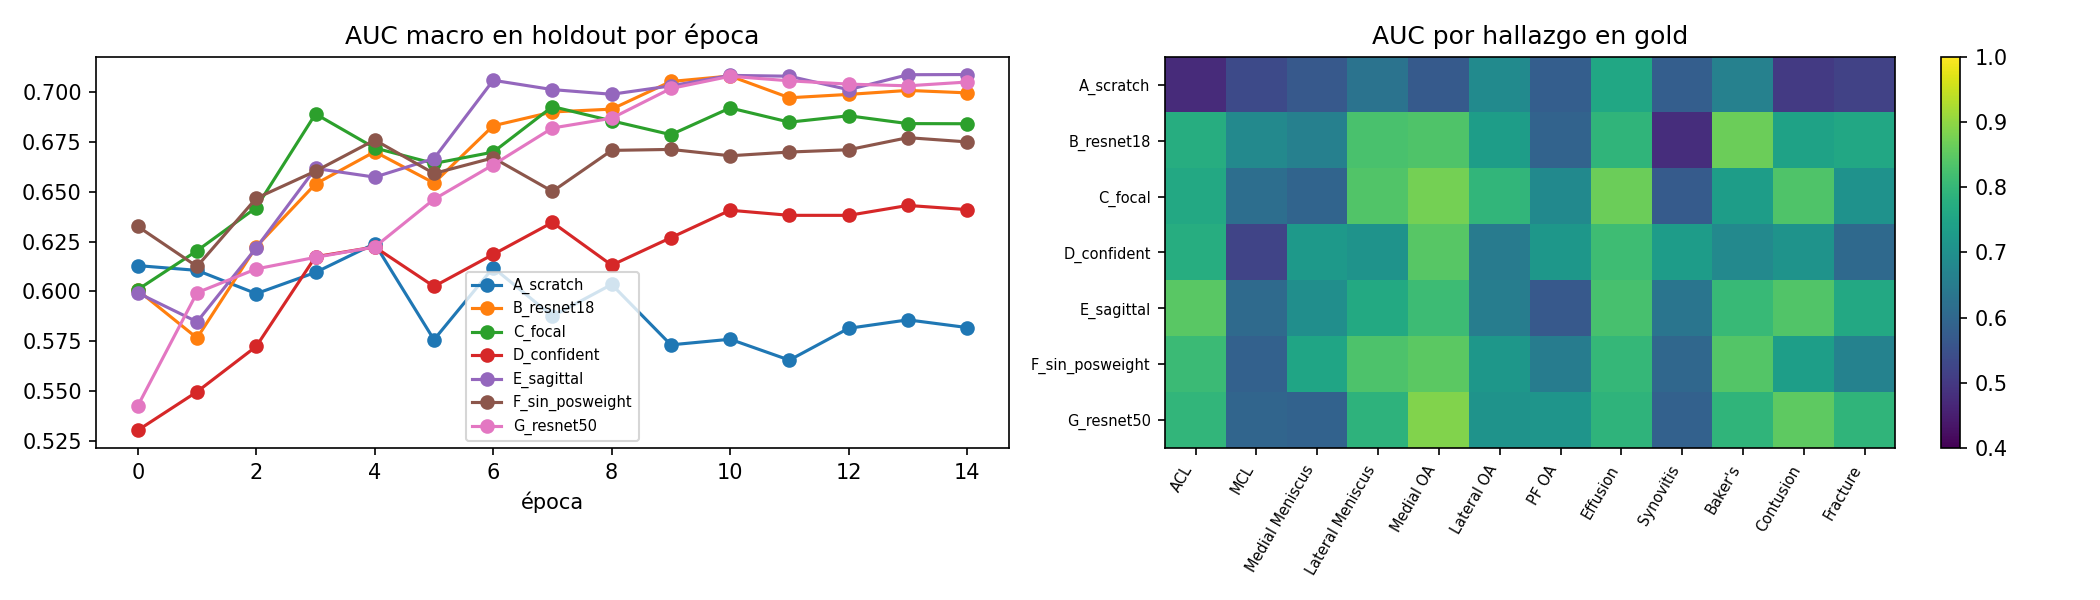
\includegraphics[width=0.92\textwidth]{figs/experimentos.png}
  \caption{Semilla 42. Izquierda: AUC macro en el holdout por época. Derecha: AUC por hallazgo en los gold para cada experimento.}
  \label{fig:experimentos}
\end{figure*}

\subsection{Estudio de ablación}
\label{sec:res-ablacion}

Cada variante C--F cambia un solo factor de B (Tabla~\ref{tab:resultados}, bloque inferior).
Con la semilla 42 ninguna diferencia es significativa: los IC pareados de C, D, E y F incluyen el cero.
Con 58 gold, diferencias de AUC menores a $\sim0.04$ no se distinguen del azar.
La desviación estándar entre semillas (0.002 a 0.010) es al menos cinco veces menor que la mitad del ancho de los IC ($\approx0.05$): la incertidumbre viene sobre todo de evaluar con 58 estudios, y repetir el entrenamiento no la reduce.
Aun así, las tres semillas separan los efectos estables del ruido:
\begin{itemize}
  \item \textbf{Pérdida focal (C):} supera a B en las tres semillas ($+0.006$ a $+0.012$) y tiene el mejor AUC medio. El efecto es consistente pero pequeño frente a los IC.
  \item \textbf{Solo etiquetas seguras (D):} descartar el silencio y la duda (peso 0) en lugar de ponderarlos queda por debajo de B en las tres semillas ($-0.022$ a $-0.052$). La pérdida depende del hallazgo: D gana en sinovitis y menisco medial, los hallazgos más sub-registrados por el reporte, porque tratar su silencio como negativo le enseña a B que casi nunca están presentes; y pierde en MCL, quiste de Baker y fractura, donde descartar el silencio deja muy pocos ejemplos (Tabla~\ref{tab:auc-hallazgo}).
  \item \textbf{Solo plano sagital (E):} rinde igual que los tres planos ($+0.004$ de media, signo variable) en el 37\% del tiempo. Es el mejor modelo en ACL (0.839), que se evalúa en el plano sagital, y pierde en artrosis patelofemoral y lateral, que se ven mejor en los planos axial y coronal.
  \item \textbf{Sin \texttt{pos\_weight} (F):} no empeora el AUC ($+0.002$ de media, de $-0.019$ a $+0.018$). Es esperable: el AUC solo mide el orden de los casos, y \texttt{pos\_weight} sobre todo desplaza la calibración, lo que el umbral elegido en el holdout compensa. En los cuatro hallazgos menos frecuentes del entrenamiento (fractura, contusión, MCL y menisco lateral), F queda a menos de 0.02 de B, mientras que C mejora en tres, sobre todo en contusión ($+0.067$).
\end{itemize}

\paragraph*{Resultados por hallazgo}
La Tabla~\ref{tab:auc-hallazgo} compara los modelos con el extractor de texto que generó sus etiquetas.
El mejor modelo de imagen de cada hallazgo supera al texto en 8 de los 12, entre ellos derrame (0.822 frente a 0.666), artrosis medial (0.886 frente a 0.760) y contusión (0.814 frente a 0.760), aunque elegir el mejor de siete modelos por hallazgo favorece a la imagen.
Un modelo entrenado con etiquetas ruidosas puede superar a su fuente cuando el ruido no es sistemático, porque la red promedia los errores individuales~\cite{ratner2017snorkel}.
En ACL, MCL, menisco medial y artrosis patelofemoral ocurre lo contrario: el reporte describe el hallazgo de forma más directa de lo que la imagen permite aprender con 540 estudios.
El AUC por hallazgo se apoya en 9 a 35 positivos y varía entre semillas con una desviación estándar de hasta 0.08 (en B, 0.079 en sinovitis, 0.061 en artrosis patelofemoral y 0.054 en MCL); la ventaja de D en sinovitis, por ejemplo, es de $+0.253$ con la semilla 42 y de $-0.010$ con la semilla 2.
Por eso las diferencias de pocas centésimas entre modelos en un mismo hallazgo no son fiables.

\begin{table*}[t]
  \caption{AUC por hallazgo en los gold, media de 3 semillas. Última columna: el extractor de texto (v4), que generó las etiquetas de entrenamiento. En negrita, el mejor modelo de imagen por hallazgo. $n^{+}$: positivos según el experto}
  \label{tab:auc-hallazgo}
  \centering
  \footnotesize
  \begin{tabular}{@{}lrccccccc|c@{}}
    \toprule
    Hallazgo & $n^{+}$ & A & B & C & D & E & F & G & Texto \\
    \midrule
    ACL              & 24 & .491 & .784 & .794 & .793 & \textbf{.839} & .814 & .795 & .885 \\
    MCL              &  9 & .531 & \textbf{.638} & .615 & .514 & .596 & .636 & .610 & .754 \\
    Medial Meniscus  & 26 & .604 & .655 & .640 & \textbf{.746} & .685 & .673 & .620 & .752 \\
    Lateral Meniscus & 23 & .603 & .804 & \textbf{.839} & .703 & .790 & .788 & .768 & .806 \\
    Medial OA        & 15 & .599 & .875 & .879 & .850 & .826 & \textbf{.886} & .881 & .760 \\
    Lateral OA       & 11 & .681 & .750 & \textbf{.759} & .635 & .696 & .725 & .708 & .733 \\
    PF OA            & 21 & .570 & .662 & .662 & .657 & .614 & \textbf{.667} & .653 & .690 \\
    Effusion         & 35 & .791 & .761 & \textbf{.822} & .802 & .789 & .768 & .800 & .666 \\
    Synovitis        & 27 & .591 & .570 & .575 & \textbf{.683} & .649 & .582 & .534 & .658 \\
    Baker's          & 12 & .643 & .826 & .778 & .720 & .785 & .814 & \textbf{.839} & .821 \\
    Contusion        & 19 & .504 & .748 & \textbf{.814} & .706 & .806 & .754 & .808 & .760 \\
    Fracture         & 18 & .535 & .715 & .728 & .581 & .767 & .706 & \textbf{.812} & .758 \\
    \midrule
    Macro            &    & .595 & .732 & \textbf{.742} & .699 & .737 & .735 & .736 & .753 \\
    \bottomrule
  \end{tabular}
\end{table*}

\paragraph*{Umbral y métricas de decisión}
El modelo final se elige sin mirar los gold: es el de mejor AUC en el holdout con la semilla 42, E (0.7087, empatado en la práctica con B y G).
La Tabla~\ref{tab:prf} muestra sus métricas con el umbral de cada hallazgo elegido en el holdout.
El \emph{recall} medio (0.73) es mayor que la precisión (0.47) porque la prevalencia de los gold difiere de la del entrenamiento (Tabla~\ref{tab:prevalencia}).

\begin{table}[t]
  \caption{Modelo final (E, elegido por holdout, semilla 42) en los gold, con umbrales que maximizan F1 en el holdout}
  \label{tab:prf}
  \centering
  \footnotesize
  \setlength{\tabcolsep}{4pt}
  \begin{tabular}{@{}lcccccc@{}}
    \toprule
    Hallazgo & Prev. & AUC & Umbral & Prec. & Recall & F1 \\
    \midrule
    ACL              & .414 & .847 & .64 & .750 & .750 & .750 \\
    MCL              & .155 & .608 & .53 & .167 & .444 & .242 \\
    Medial Meniscus  & .448 & .696 & .20 & .491 & 1.00 & .658 \\
    Lateral Meniscus & .397 & .764 & .08 & .543 & .826 & .655 \\
    Medial OA        & .259 & .811 & .26 & .361 & .867 & .510 \\
    Lateral OA       & .190 & .654 & .11 & .211 & .727 & .327 \\
    PF OA            & .362 & .568 & .20 & .358 & .905 & .514 \\
    Effusion         & .603 & .825 & .43 & .660 & .943 & .776 \\
    Synovitis        & .466 & .633 & .61 & .667 & .222 & .333 \\
    Baker's          & .207 & .804 & .27 & .300 & 1.00 & .462 \\
    Contusion        & .328 & .837 & .78 & .600 & .789 & .682 \\
    Fracture         & .310 & .761 & .84 & .545 & .333 & .414 \\
    \midrule
    Media            &      & .734 &     & .471 & .734 & .527 \\
    \bottomrule
  \end{tabular}
\end{table}

\subsection{Interpretabilidad y análisis de errores}
\label{sec:res-gradcam}

La Fig.~\ref{fig:gradcam} aplica Grad-CAM~\cite{selvaraju2017gradcam} al modelo final en cuatro hallazgos.
Solo el mapa del derrame es anatómicamente plausible: cubre la cavidad articular y el receso anterior al fémur.
El del menisco medial parte de la línea articular, donde está el menisco, pero se extiende hacia la diáfisis tibial.
Los de ACL y quiste de Baker no señalan la estructura correcta: el de ACL se concentra en la región suprarrotuliana anterior y no en la escotadura intercondílea, y el de Baker en la grasa de Hoffa, en la cara anterior, mientras que el quiste poplíteo es posterior.
Una explicación plausible es un atajo por co-ocurrencia: la rotura aguda de ACL suele acompañarse de derrame (hemartrosis) y el quiste de Baker comunica con el líquido articular, de modo que, como las etiquetas salen del mismo reporte, el modelo puede predecirlos a partir del líquido, que es más fácil de ver.
El AUC de ACL (0.847) sería entonces en parte un efecto de correlación.
Además, Grad-CAM en la última capa de ResNet tiene una resolución de $7\times7$, por lo que la localización es gruesa.

Los errores se concentran donde la supervisión es más débil o se desplaza.
MCL (9 positivos) y artrosis patelofemoral tienen los AUC más bajos.
En sinovitis y fractura, que en los gold son el doble de frecuentes que en el entrenamiento, el umbral elegido con la prevalencia débil deja el \emph{recall} en 0.22 y 0.33 (Tabla~\ref{tab:prf}).

\begin{figure*}[t]
  \centering
  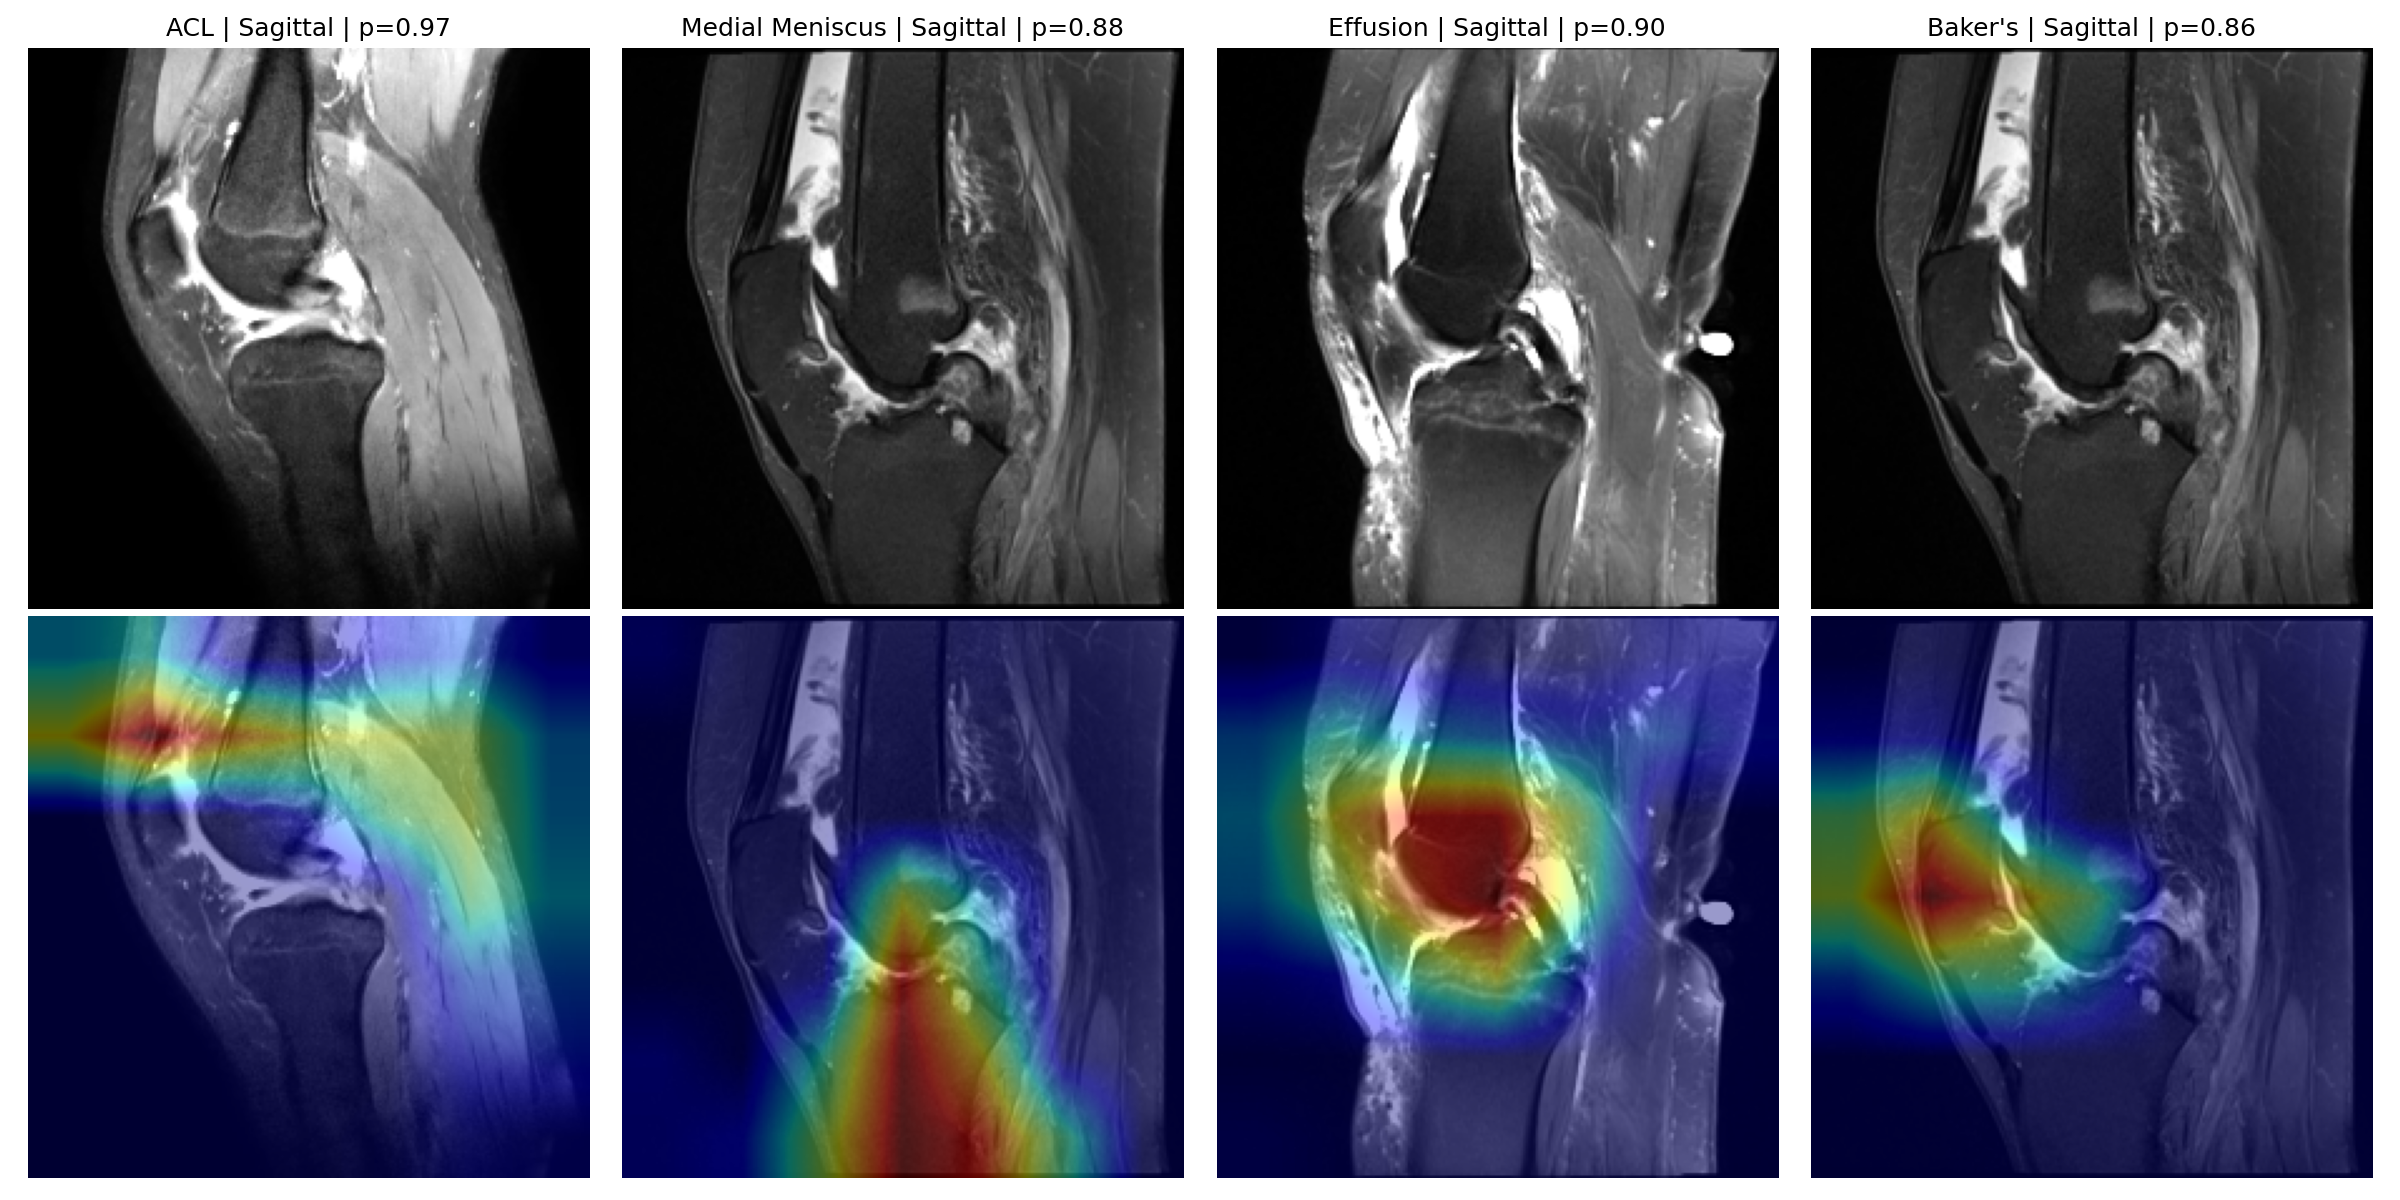
\includegraphics[width=0.85\textwidth]{figs/gradcam.png}
  \caption{Grad-CAM del modelo final (E) sobre su última capa convolucional, en la ventana con mayor atención para cada hallazgo y un estudio gold positivo. Anterior está a la izquierda.}
  \label{fig:gradcam}
\end{figure*}

\subsection{Costo computacional}
\label{sec:res-costo}

Todo el entrenamiento se hizo en una GPU NVIDIA T4 de Kaggle.
La primera corrida (7 entrenamientos) tomó 49 min y la segunda (21 entrenamientos), 153 min: en total, unas 3.4 horas de GPU, más una prueba previa de una época.
Por entrenamiento, ResNet-18 tarda $\approx$5 min, ResNet-50 13.4 min y la variante sagital 1.9 min (Tabla~\ref{tab:resultados}).
La prueba previa mostró que la primera lectura de la caché desde disco dominaba el tiempo (673 s frente a 24 s por época), por lo que los volúmenes usados se cargan una sola vez en RAM.
El preprocesamiento de los 4407 estudios genera una caché de 10.6\,GB y corre en CPU.
El tiempo de inferencia por estudio no se midió por separado: está incluido en los $\approx$24 s por época de B, que abarcan el entrenamiento y la evaluación de los 60 estudios del holdout.

% ---------------------------------------------------------------------------
\section{Discusión}
\label{sec:discusion}

\paragraph*{Por qué funciona y qué dicen la ablación y Grad-CAM}
El método funciona en la medida en que lo permiten sus etiquetas.
El preentrenamiento es lo único que cambia el resultado de forma clara, porque con 540 estudios ruidosos la red no puede aprender rasgos visuales desde cero.
Las demás decisiones (pérdida, planos, profundidad, reponderado) mueven el AUC macro menos que el ruido de evaluación; la ablación con tres semillas solo separa dos efectos estables y pequeños: la focal ayuda y descartar las etiquetas inciertas perjudica.
Que la variante sagital rinda igual en el 37\% del tiempo y que Grad-CAM apunte al líquido articular en ACL y Baker indican lo mismo: el modelo aprende las regularidades más fáciles de la imagen que se correlacionan con el reporte, no necesariamente la anatomía de cada lesión.

\paragraph*{Comparación con lo publicado}
MRNet~\cite{bien2018mrnet} reporta un AUC de 0.965 para rotura de ACL entrenando con 1130 estudios con etiquetas expertas, frente a 0.78--0.84 aquí con etiquetas débiles (media de tres semillas, Tabla~\ref{tab:auc-hallazgo}).
Las soluciones públicas de la competencia reportan entre 0.89 y 0.96 en el \emph{leaderboard}~\cite{pilkwang2026baseline,dread2026twelve,ab29knee,bishnoi2026rsna}, con todos los estudios, \emph{backbones} más grandes y ensambles.
Esas cifras se miden en el conjunto de prueba oculto y no son directamente comparables con las de los 58 gold, pero indican que el margen de mejora está en los datos y la escala, no en la cabeza de atención.

\paragraph*{Limitaciones}
Los 58 gold miden tanto el extractor como el modelo, y dos parámetros del extractor (derrame leve $=0.5$ y sinovitis leve $=1$) se fijaron mirándolos, lo que puede hacer algo optimista la evaluación.
Con 58 estudios, los IC tienen un ancho cercano a $\pm0.05$ y el AUC de cada hallazgo se apoya en 9 a 35 positivos.
El modelo se entrenó con 600 de los 4349 estudios disponibles y una sola partición, y su validez externa en otros escáneres y hospitales no se evaluó.
El preprocesamiento no normaliza la lateralidad, no recorta a una extensión física fija y usa una sola serie por plano.

\paragraph*{Sesgos, riesgos y privacidad}
El extractor produce más silencio en algunos idiomas (español, griego, neerlandés), lo que significa más falsos negativos en las etiquetas de esos centros y, por tanto, un modelo peor calibrado para su población.
Para un uso en el Perú, donde los reportes están en español, este sesgo tendría que corregirse antes de cualquier aplicación.
Además, los gold tienen el doble de prevalencia de fractura, contusión y sinovitis que las etiquetas débiles, así que los umbrales no se trasladan a una población con otra mezcla de casos.
Un modelo que aprende atajos por co-ocurrencia puede fallar justo en los casos atípicos, por lo que no debe usarse para diagnóstico sin validación clínica.
Se trabajó solo con los datos publicados para la competencia, identificados por UID, y no se intentó vincularlos con otras fuentes.

% ---------------------------------------------------------------------------
\section{Conclusiones}
\label{sec:conclusiones}

En la detección de hallazgos de rodilla con etiquetas débiles, la calidad de la supervisión domina sobre la arquitectura.
Un extractor de reglas multilingüe permite entrenar sin etiquetas expertas y un modelo de imagen que se acerca a él e incluso lo supera en hallazgos con ruido no sistemático, pero hereda sus omisiones: lo que el radiólogo no escribe, como la sinovitis, el modelo no lo aprende, y lo que co-ocurre en el reporte, como derrame y rotura de ACL, el modelo lo confunde.
Con la escala de este trabajo, solo el preentrenamiento produce una diferencia significativa, y repetir con varias semillas es necesario para no confundir el ruido con un efecto, sobre todo por hallazgo.

Como trabajo futuro, en orden de impacto esperado según las soluciones públicas: normalizar la lateralidad invirtiendo el eje medial-lateral de las rodillas izquierdas y recortar a unos 130\,mm antes de redimensionar~\cite{pilkwang2026baseline}; entrenar con los 4349 estudios y validación cruzada de 5 particiones; limpiar las etiquetas con un esquema \emph{teacher-student}~\cite{ab29knee}; y usar \emph{backbones} más fuertes a mayor resolución.

% ---------------------------------------------------------------------------
\section*{Contribuciones}

% Tareas por integrante pendientes de confirmar.
\begin{table}[h]
  \centering
  \footnotesize
  \begin{tabular}{@{}lp{0.48\columnwidth}@{}}
    \toprule
    Integrante & Tareas en las que participó \\
    \midrule
    Burgos Choquehuanca Juan      & Por completar \\
    Paredes Abanto Davis Roberto  & Por completar \\
    Salguero Torres Carlos Adrian & Por completar \\
    Ramirez Quispe Huber Angel    & Por completar \\
    \bottomrule
  \end{tabular}
\end{table}

\section*{Disponibilidad de código y uso de herramientas de IA}

El código, los resultados y este informe están en \url{https://github.com/hramirezq/rsna-knee-abnormality-detection}.
Los pesos (\texttt{ckpt\_*.pt}, $\approx$840\,MB) no se versionan por su tamaño; se regeneran ejecutando el notebook en Kaggle en modo \texttt{train}.
Se usó Claude Code (Anthropic) como asistente para depurar y revisar el código del notebook, analizar los resultados y redactar y maquetar este informe; los resultados se verificaron contra los archivos generados por el notebook.

\bibliographystyle{IEEEtran}
\bibliography{referencias}

\end{document}
